\documentclass[a4paper]{article}
\usepackage{graphicx} % Required for inserting images
\graphicspath{{./images/}}


%% Language and font encodings
\usepackage[english]{babel}
\usepackage[utf8x]{inputenc}
\usepackage[T1]{fontenc}
\usepackage{booktabs}
\usepackage{algorithm}
\usepackage{algorithmicx}
\usepackage{amsfonts}
\usepackage[noend]{algpseudocode}
\usepackage{color,soul}
\usepackage{multicol}
\usepackage{amsmath}
\usepackage{amssymb}
\usepackage{wrapfig}
\usepackage{hyperref}



\usepackage{courier} %% Sets font for listing as Courier.
\usepackage{listings, xcolor}
\lstset{
tabsize = 4, %% set tab space width
showstringspaces = false, %% prevent space marking in strings, string is defined as the text that is generally printed directly to the console
numbers = left, %% display line numbers on the left
commentstyle = \color{orange}, %% set comment color
keywordstyle = \color{blue}, %% set keyword color
stringstyle = \color{red}, %% set string color
rulecolor = \color{black}, %% set frame color to avoid being affected by text color
basicstyle = \small \ttfamily , %% set listing font and size
breaklines = true, %% enable line breaking
numberstyle = \tiny,
}

%%damit I.H über = steht
\newcommand\myEqualOne{\mathrel{\overset{\makebox[0pt]{\mbox{\normalfont\tiny\sffamily I.H}}}{=}}}


%% Sets page size and margins
\usepackage[a4paper,top=3cm,bottom=2cm,left=3cm,right=3cm,
            marginparwidth=1.75cm]{geometry}

%%--------------------------begin Document--------------------------------
\title{Algorithmen und Datenstrukturen 2023}
\author{bergery@student.ethz.ch}
\date{Oktober 2023}

\begin{document}
\maketitle
\begin{center}
    
\includegraphics{Pictures/eth_logo_kurz_pos Kopie.png}
\end{center}

\tableofcontents
\newpage

%%Chapter 01
\section{Vorwort}
Dieses Skript dient dazu eine grobe Übersicht für die Vorlesung "Algorithmen und Datenstrukturen" zu geben. Jegliches aufgeführte Informationen sollte man an der Prüfung können.\\
Für etliche Fehler in diesem Skript wird keine Verantwortung übernommen.

%%Chapter 02
\section{Mathematische Grundlagen}
\subsection{Induktion}
    Die vollständige Induktion ist eine mathematische Beweismethode, nach der eine Aussage für alle natürlichen Zahlen bewiesen wird, die größer oder gleich einem bestimmten Startwert sind. Da es sich um unendlich viele Zahlen handelt, kann eine Herleitung nicht für jede Zahl einzeln erbracht werden. Sie ist ein deduktives Verfahren. \\
    Der Beweis, dass die Aussage $A(n)$ für alle $n \geq n_0 (n_0$ meist 0 oder 1), gilt, wird dabei in zwei Etappen durchgeführt:
    \begin{enumerate}
        \item Im \textit{Induktionsanfang} wird die Gültigkeit der Aussage $A(n_0)$ für eine kleinste Zahl $n_0$ gezeigt.
        \item Im \textit{Induktionsanfang} wird für ein beliebiges $n \geq n_0$ die Gültigkeit der Aussage $A(n+1)$ aus der Gültigkeit von $A(n)$ geschlussfolgert.
    \end{enumerate}
    \textbf{Beispiel:} \\
        Aussage: $A(n):= 1 + 2 + 3 + ...+ n = \frac{n \cdot (n+1)}{2}$ für $n \geq 1$ \\
        \textit{Base Case}: Für $n = 1$ gilt: $1 = \frac{1 \cdot (1+1)}{2} \rightarrow 1 = 1 \ \checkmark$ \\
        \textit{Induction hypothesis}: "We now assume that it is true for $n = k$, i.e., $1 + 2 + 3 + ...+ k = \frac{k \cdot (k+1)}{2} $.
        \textit{Induction step}: $k \rightarrow k+1$ \\
        $1 + 2 + 3 + ...+ k + (k+1) \myEqualOne  \frac{k \cdot (k+1)}{2} + (k+1)$, where $\frac{k \cdot (k+1)}{2} + (k+1) = \frac{k^2 + 3k + 2}{2} = \frac{(k+1) \cdot (k+2)}{2} \ \square.$
        By the principle of mathematical induction, we conclude that $ 1 + 2 + 3 + ...+ n = \frac{n \cdot (n+1)}{2}$ is true for all $n \in \mathbb{N}.$
        \\
        
    \subsection{Wichtige Annäherungen}
    Damit wir schnelle Resultate erhalten können, sind Approximationen ein fundamentaler Bestandteil. Aus diesem Grund folgende Liste:

    \begin{itemize}
        \item  $n! \leq n^n, $ for $  n\geq 1 $
        \item $\big(\frac{n}{2}\big)^{{n}/{2}} \leq n!, \ for\ n\geq 1 $
        \item $ \sum_{i=0}^{n} \log n  = \ \log\prod_{i=1}^{n}n = \log{n!} \ \approx n\log n \to\mathcal{O}(n \log n)$
        \item $\sum_{i=0}^{n} 1 = (n+1)  \to \mathcal{O}(n)$
        \item $\sum_{i=0}^{n} i = \frac{n(n+1)}{2} \to \mathcal{O}(n^2)$
        \item $\sum_{i=0}^{n} i^2 = \frac{n(n+1)(2n+1)}{6} \to \mathcal{O}(n^3)$
        \item $\sum_{i=0}^{n} i^3 = \frac{n^2(n+1)^2}{4}  \to\mathcal{O}(n^4)$
        \item binomial coefficient: $\binom{n}{k}= \frac{n!}{k!(n-k)!}$
        \item $\binom{n}{0}=\binom{n}{n}=1  \quad\quad
              \binom{n+1}{k+1}=\binom{n}{k}+\binom{n}{k+1}  \quad\quad
              \binom{n}{n-k}=\binom{n}{k}$
        \item $\sum_{i=1}^{n}i^k \leq \sum_{i=1}^{n}n^k$
    \end{itemize}
        

    \subsection{Big-O Notation}
    Landau-Symbole (engl. Big-O notation) werden verwendet, um das asymptotische Verhalten von Funktionen und Folgen zu beschreiben.
    In der Informatik werden sie bei der Analyse von Algorithmen verwendet und geben ein Maß für die Anzahl der Elementarschritte oder der Speichereinheiten in Abhängigkeit von der Größe des gegebenen Problems an. \\
    Für Annäherungen wird auch sehr oft die \textbf{Regel von de l'Hôpital} \label{Hopital} angewendet:\\
        Let $f, g : \mathbb{R}\to\mathbb{R}$ be differentiable functions with $f(x)\to\infty, g(x)\to\infty$ for $x\to\infty$. \\
        If $\lim_{x\to\infty}\frac{f'(x)}{g'(x)}$ exists, then
        $\lim_{x\to\infty}\frac{f(x)}{g(x)}=\lim_{x\to\infty}\frac{f'(x)}{g'(x)}$


    

    \subsubsection{Definition O-Notation}
    In der Tabelle (\ref{tab:ONotation}) sehen wir jegliche Definition der $\mathcal{O}$-Notation.
    Wir unterscheiden zwischen, $\Omega$ (Omega) [lower-bound], $\Theta$ (Theta) [tight-bound] und  $\mathcal{O}$ [upper-bound]. Damit dies noch mathematisch formuliert ist haben wird folgendes: \\
    Let $f, g: \mathbb{R} \rightarrow \mathbb{R}^+$ such that the limit of $\frac f g$ exists. Then:
    
    \begin{equation*}
    \lim_{x\to\infty}\frac fg = \infty \Rightarrow g \in \mathcal{O}(f) \text{and} f \in \Omega(g)
    \end{equation*}
    \begin{equation*}
    \lim_{x \rightarrow \infty} \frac fg = C \in \mathbb{R}^+ \setminus \left\lbrace 0 \right\rbrace \Rightarrow f \in\Theta(g)  \text{and } g \in\Theta(f) \\
    \end{equation*}
    \begin{equation*}
    \lim_{x \rightarrow \infty} \frac fg = 0 \Rightarrow f \in\mathcal{O}(g) \text{and } g \in\Omega(f) \\
    \end{equation*}


    \begin{table}
        \centering
        \small
        \begin{tabular}{c|c|c}
            Notation & Definition & Mathematische Definition \\
            \hline
            $f \in o(g)$ 
            & asymptotisch gegenüber $g$ vernachlässigbar 
            & $\lim_{x\to a} \big| \frac{f(x)}{g(x)} \big| = 0 $\\
            
             $f \in \mathcal{O}(g)$
             & asymptotische obere Schranke  
             & $\limsup_{x\to a} \big| \frac{f(x)}{g(x)} \big| < \infty $ \\
             
            $f = \Omega(g)$ 
            & asymptotische untere Schranke, $f$ ist nicht in $o(g)$ 
            & 
            $\limsup_{x\to a} \big| \frac{f(x)}{g(x)} \big| > 0 $\\

            $f \in \Theta(g)$            
            & scharfe Schranke,  sowohl $f \in \mathcal{O}(g)$ als auch $f \in \Omega(g)$
            &  $0 < \liminf_{x\to a} \big| \frac{f(x)}{g(x)} \big| \leq \limsup \big| \frac{f(x)}{g(x)} \big| < \infty $ \\

            $f \in \omega(g)$
            &  asymptotisch dominant, $g \in o(f)$
            & $\lim_{x \to a}\frac{f(x)}{g(x)} \big| = \infty$ \\
        \hline
        \end{tabular}
        \caption{Definition der $\mathcal{O}$-Notation}
        \label{tab:ONotation}
    \end{table}
    
    \subsubsection{Master Theorem}
    Damit das Rechnen mit solchen Grenzwerten schneller geht, haben wir das Master-Theorem, welches sehr praktische Anwendung mit sich bringt:
      \begin{equation} \label{MasterTheorem}
  T(n) \leq aT(n/2)\ + Cn^b: =\begin{cases}      T(n) \leq \mathcal{O}(n^b), & \text{b >} \log_2(a)\\
      T(n) \leq \mathcal{O}(n^b\log(n)) &\text{b =} \log_2(a)\\
      T(n) \leq \mathcal{O}(n^{\log_2(a)}) & \text{b <} \log_2(a)
    \end{cases}         
  \end{equation}

    \subsubsection{Overview}
    Damit wir nun einmal sehen können wie die asympotischen Grenzen sich verhalten, folgende Abbildung: 
    \begin{figure}[h]
        \centering
        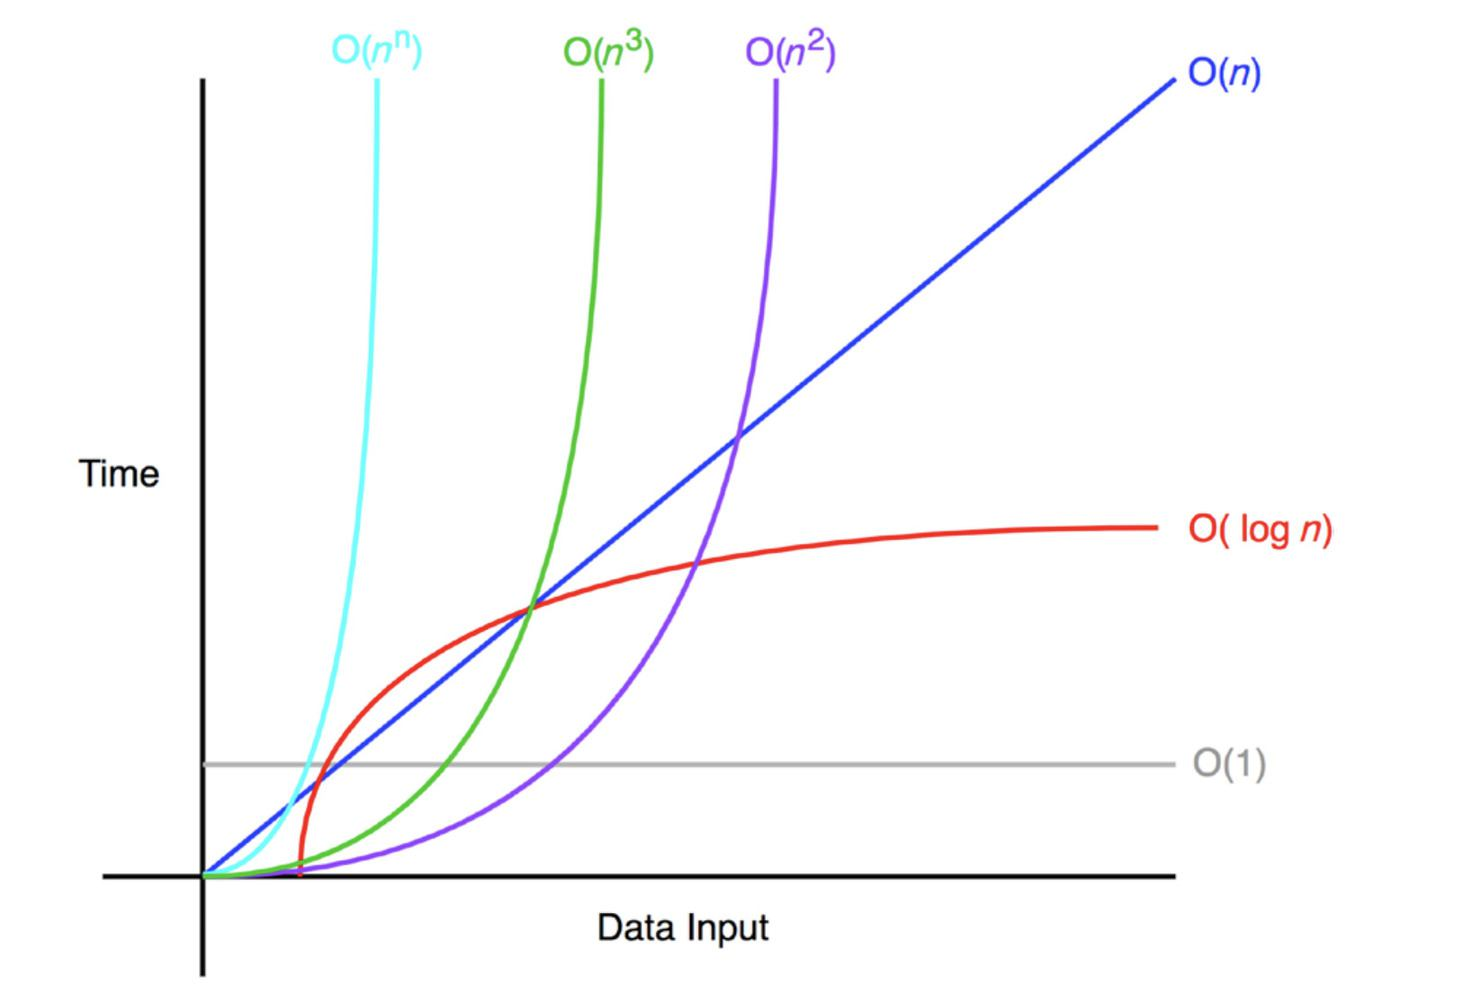
\includegraphics[width=0.4\textwidth]{Pictures/big-o-notation.jpg}
        \caption{Wachstum verschiedener Funktionen}
        \label{fig: WachstumBigO}
    \end{figure}
    Die graphische Darstellung der Funktionen im Bild (\ref{fig: WachstumBigO}) zeigt uns leider nur sechs Funktionen. 
    Um möglichst viele Funktionen in aufsteigendem, asymptotischen Wachstum zu sehen, folgende Abbildung:

    $\mathcal{O}(1) \in  \mathcal{O}(\log \log n)\in \mathcal{O}(\log n) \in \mathcal{O}(\sqrt{n}) \in \mathcal{O}(n) \in \mathcal{O}(n\log n) \in \mathcal{O}(n^2) \in \mathcal{O}(2^n) \in \mathcal{O}(2^{n^{2}}) \in \mathcal{O}(n!) $
\newpage
\subsection{Erster Algorithmus}
    \subsubsection{Maximum Subarray Sum}
    Für einen ersten Algorithmus schauen wir den \texttt{Maximum Subarray Sum} Algorithmus an. Dieser Algorithmus enthält ein Array von $n$ rationalen Zahlen $a_1,..., a_n$ und gesucht ist ein Teilstück mit maximaler Summe.  \\
    \textbf{Beispiel}: \\
    Sei ein Array [-2, -5, 6, -2, -3, 1, 5, -6] gegeben, so ist die maximale Teilsumme dieses Array 7, nämlich $ 6 + (-2) + (-3) + 1 + 5 = 7$. \\

\begin{algorithm}
    \caption{Maximum Subarray Sum $(a_1,..., a_n)$}\label{MSS-1}
\begin{algorithmic}
        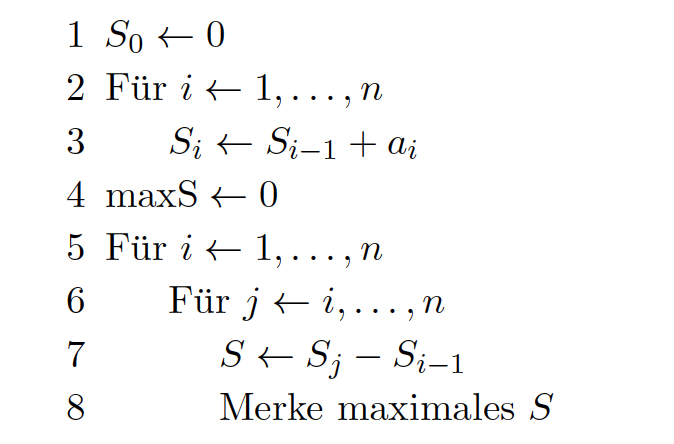
\includegraphics[scale = 0.39]{Pictures/MSS-naiv.png}

    \end{algorithmic}
    
\end{algorithm}

Dieser naive Algorithmus führt insgesamt $\Theta(n^3)$ viele Additionen aus, was sehr schlecht ist für unseren Algorithmus.
\begin{algorithm}
 \caption{MSS divide and conquer $(a_1,..., a_n)$}\label{MSS-DivAQ}
    \begin{algorithmic}
         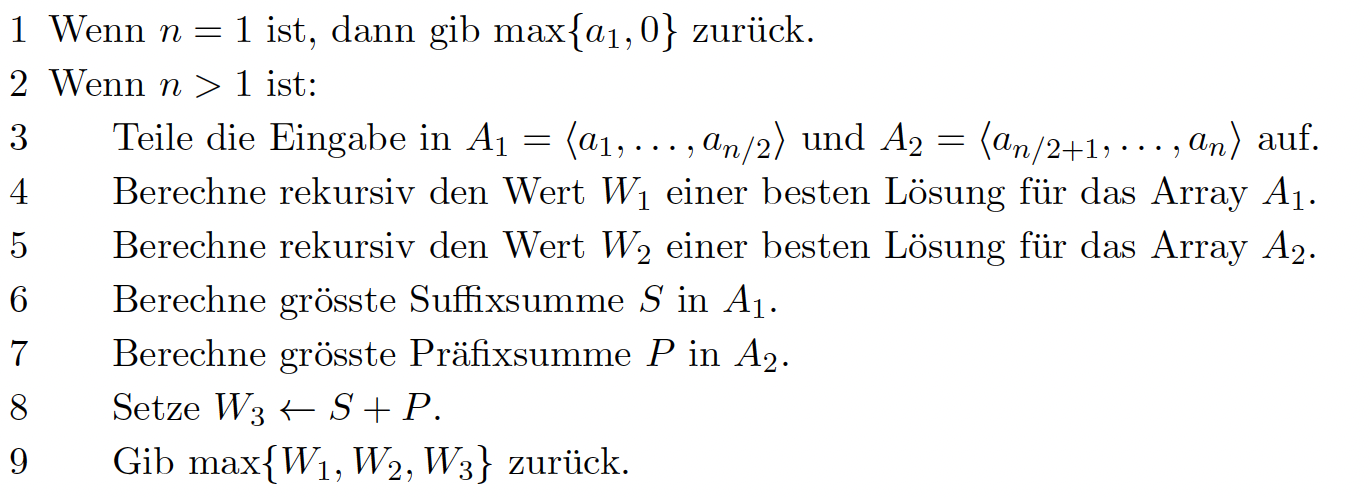
\includegraphics[scale = 0.4]{Pictures/MSS-DivandConq.png}
    \end{algorithmic}
\end{algorithm}

    Wir haben schon eine Verbesserung des Algorithmus von $\Theta(n^3)$ vielen Additionen zu $\Theta(n\log n)$ vielen Additionen. In einem letzten Schritt können wir diesen sogar noch einmal verbessern nämlich bis zu $\Theta(n)$ viele Additionen.

\begin{algorithm}
 \caption{MSS-Induktiv $(a_1,..., a_n)$}\label{MSS-Induktiv}
    \begin{algorithmic}
         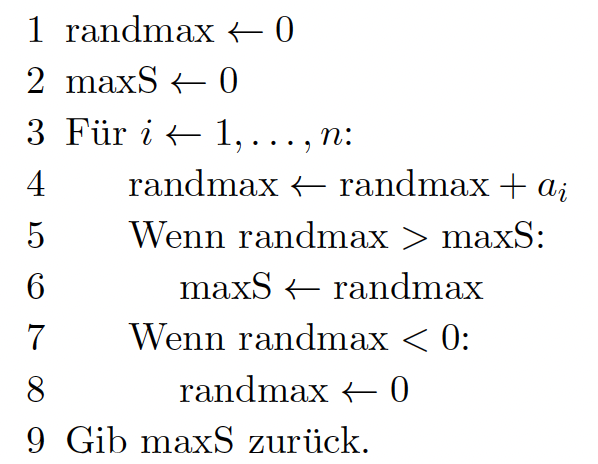
\includegraphics[scale = 0.39]{Pictures/MSS-Induktiv.png}
    \end{algorithmic}
\end{algorithm}

\newpage
%%Chapter 03
\section{Suchen und Sortieren}
\subsection{Suchen}
    In diesem Abschnitt schauen wir wie schnell wir in abstrakten Daten Strukturen suchen, einfügen und löschen können. Die meist gebrauchten Datenstrukturen sind somit in folgender Tabelle aufgeführt mit ihrer korrespondierender Laufzeit: \\
\begin{center}      
\begin{tabular} {|c|c|c|c|}
  \hline
  \label{Tab: LaufzeitenSuchSortier}
  \bfseries Data structure & \bfseries Search & \bfseries Insert & \bfseries Delete\\
  \hline
  Unsorted Array	&$O(n)$				&$O(1)$			&$O(n)$\\
  Sorted Array		&$O(\log{n})$	          	&$O(n)$			&$O(n)$\\
  Unsorted List 	&$O(n)$				&$O(1)$			&$O(n)$\\	
  Sorted List		&$O(n)$				&$O(n)$			&$O(n)$\\	
  Unbalanced Tree	&$O(n)$				&$O(n)$			&$O(n)$\\
  AVL tree		&$O(\log{n})$	        	&$O(\log{n})$	        &$O(\log{n})$\\
  \hline
\end{tabular}
\end{center}  
Wir stellen fest, dass es im Allgemeinen einen Kompromiss gibt zwischen einfachen Datenstrukturen, die ein einfaches Einfügen und Löschen ermöglichen, aber die Einträge nicht vorverarbeiten, um spätere Suchvorgänge zu erleichtern (ungeordnetes Array), und komplexeren Datenstrukturen mit höheren Einfüge- und Löschkosten, die effizienter abgefragt werden können.

\subsubsection{Binary Search} \label{BinarySearch}
    Binary Search ist der standart Suchalgorithmus für \textbf{sortierte} Arrays, da es einen effizienten, logarithmische Laufzeitkomplexität hat.

\begin{algorithm}
\caption{Binary search} 
\begin{algorithmic}
  \Function{FindIndex}{$A$, $e$} \Comment{Search item $e$ in sorted array $A$}
  \State $l, r \gets 0, A\texttt{.length}-1$
  \While{$r > l$}
  \State $m \gets \left\lfloor \frac{l+r}{2} \right\rfloor$
  \If{$A\left[m\right] = e$}
  \State \Return $m$
  \ElsIf{$A\left[m\right] > e$}
  \State $r \gets m-1$
  \Else
  \State $l \gets m+1$
  \EndIf
  \EndWhile
  \State \Return \texttt{"not found"}
  \EndFunction
\end{algorithmic}
\end{algorithm}
Obwohl bei der binären Suche die Kosten für die Suche in geordneten Arrays logarithmisch werden, sind Einfügung und Löschung immer noch linear: im schlimmsten Fall, d.h. wenn das einzufügende oder zu löschende Element das erste Element des Arrays ist, müssen wir alle Elemente um einen Schritt nach rechts/links verschieben.

\subsubsection{Heaps}
Noch effizienter als geordnete Arrays sind daher baumartige Strukturen, bei denen die Kosten für das Einfügen und Löschen ebenfalls logarithmisch sein können. Heaps sind eine spezielle Klasse von baumbasierten Strukturen, die eine effiziente (zeitkonstante) Methode zur Extraktion des kleinsten oder größten Elements bieten.

Genauer gesagt sind Min- (bzw. Max-) Heaps baumbasierte Datenstrukturen, die die folgende Heap-Invariante erfüllen: Wenn $A$ das Elternteil von $B$ ist, dann ist der Wert von Knoten $A$ kleiner (bzw. größer) als der Wert von Knoten $B$. Wir betrachten hier binäre Min-Heaps, was bedeutet, dass ein Elternteil einen kleineren Wert hat als seine (höchstens zwei) Kinder. Für binäre Min-Haufen gilt zusätzlich die folgende Forminvariante: Der betrachtete Haufen ist immer ein vollständiger binärer Baum, d. h. alle Schichten des Baums sind von oben nach unten und von links nach rechts gefüllt.


\begin{figure}[h] 
\caption{Beispiel eines Min-Heaps}
\centering
\label{fig: Min-heap}
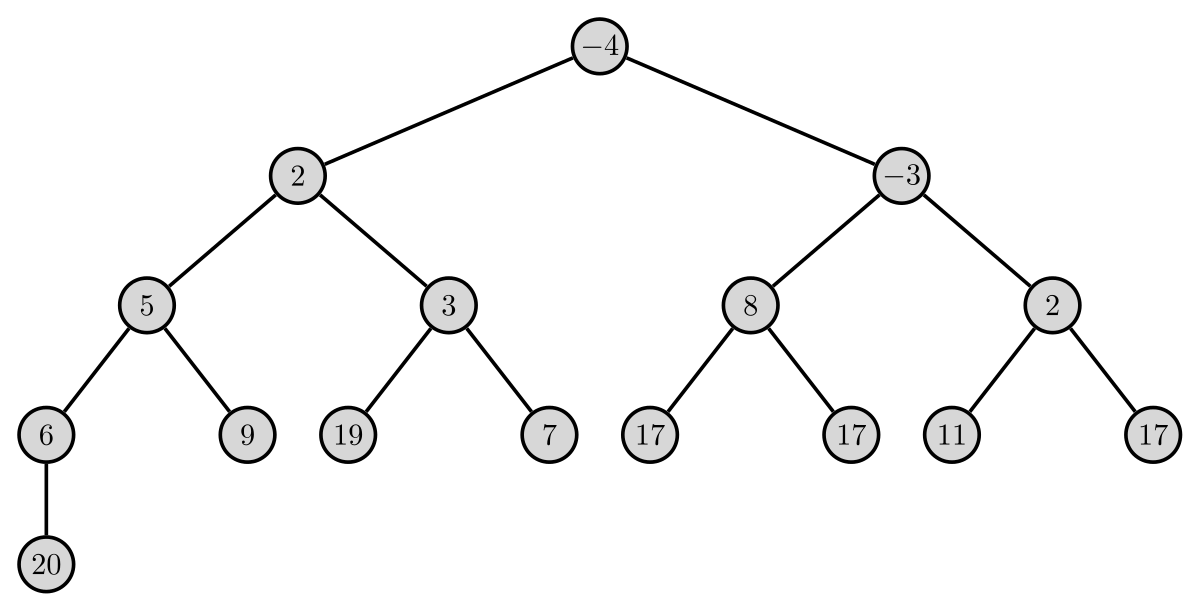
\includegraphics[scale= 0.2]{Pictures/Heap.svg.png}
\end{figure}

\begin{figure}[h] 
\caption{Beispiel 0-Heaps}
\centering
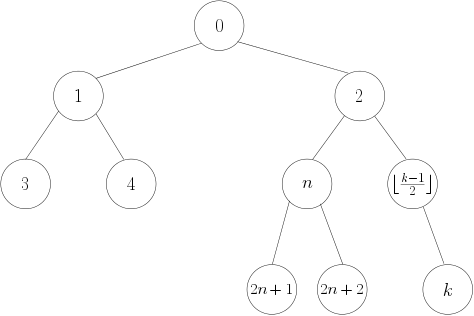
\includegraphics[scale= 0.5]{Pictures/0-heap.png}
\label{fig: 0-Heap}
\end{figure}



\subsubsection*{Implementation}
Die gebräuchlichste Implementierung ist ein Array (mit fester oder dynamischer Größe). Geht man von einem 0-basierten Array aus (vgl. Figure \ref{fig: 0-Heap}), so sind die \textit{children} des Knotens $n$, $2n+1$ und $2n+2$ und die \textit{parent} des Knotens $k$ ist der Knoten $\lfloor \frac{k-1}{2}\rfloor$.


\subsubsection*{Common operations}
Here are the most common operations that a min-heap must support:
\begin{itemize}
\item \textbf{Basic operations}
  \begin{itemize}
  \item Find min,
  \item Delete min,
  \item Insert,
  \item Find min and delete it (pop);
  \end{itemize}
\item \textbf{Initialization}
  \begin{itemize}
  \item Create empty heap,
  \item Heapify (transform array into heap);
  \end{itemize}
\item\textbf{Inspection}
  \begin{itemize}
  \item Return size,
  \item Test if empty;
  \end{itemize}
\item \textbf{Other}
  \begin{itemize}
  \item Increase/decrease,
  \item Delete,
  \item Restore heap invariant,
  \item Merge/union.
  \end{itemize}
\end{itemize}


\subsubsection*{Preserving the heap invariant}
Die Heap Invariante sagt uns eigentlich aus: 
\begin{quote}
    "Das Label jedes Knoten $n$ ist kleiner oder gleich den Labels der Kinder von $n$."
\end{quote}
Bei der Aktualisierung eines Heaps ist es wichtig, die oben beschriebene Invariante beizubehalten. Nach einer Löschung oder einer Einfügung kann es vorkommen, dass ein (einzelnes) Element kleiner wird als eines seiner Kinder; wir können dann die Heap-Invariante in logarithmischer Zeit wiederherstellen, indem wir dieses Element nach unten durchsickern lassen.

\begin{algorithm}
\caption{Restore heap invariant by percolating element down}
\begin{algorithmic}
  \Function{PercolateDown}{$H$, $i$} \Comment{Percolate element $i$ in $H$}
  \State $e \gets H\left[i\right]$
  \If{$2i+2 = H\texttt{.length}$}
  \If{$e > H\left[2i+1\right]$}
  \State Swap $H\left[i\right]$ and $H\left[2i+1\right]$
  \EndIf
  \ElsIf{$2i+2 < H\texttt{.length}$}
  \State $l, r \gets H\left[2i+1\right], H\left[2i+2\right]$
  \If{$l < r$}
  \If{$l < e$}
  \State Swap $H\left[i\right]$ and $H\left[2i+1\right]$
  \State \textsc{PercolateDown}$\left(H, 2i+1\right)$
  \EndIf
  \Else
  \If{$r < e$}
  \State Swap $H\left[i\right]$ and $H\left[2i+2\right]$
  \State \textsc{PercolateDown}$\left(H, 2i+2\right)$
  \EndIf
  \EndIf
  \EndIf  
  \EndFunction
\end{algorithmic}
\end{algorithm}

\subsubsection*{Costs}

In der folgenden Tabelle sind die Kosten von Standard-Heap-Operationen für drei Arten von Heaps zusammengefasst: binäre Heaps, binomische Heaps und Fibonacci-Heaps. \\

\begin{tabular}{|c|c|c|c|}
  \hline
  \label{Tab: KostenHeaps}
\textbf{Operation}    & \textbf{Binary}             & \textbf{Binomial}         & \textbf{Fibonacci}   \\
\hline
search min   & $\Theta(1)$        & $\Theta(1)$      & $\Theta(1)$ \\
delete min   & $\Theta(\log n)$   & $\Theta(\log n)$ & $O(\log n)$ \\
insert       & $\Theta(\log n)$   & $\Theta(1)$      & $\Theta(1)$ \\
increase key & $\Theta(\log n)$   & $\Theta(\log n)$ & $\Theta(1)$ \\
  union        & $\Theta(m \log n)$ & $O(\log n)$      & $\Theta(1)$  \\
                                                         \hline
\end{tabular}


\subsubsection*{Zusammenfassung- Youtube}
\href{https://www.youtube.com/watch?v=0wPlzMU-k00}{Kurze Zusammenfassung anschauen}

\subsection{AVL-Trees}

\subsection{Sortier-Algorithmen}

    \subsubsection{Bubblesort}\label{alg:Bubblesort}
    

    \subsubsection{Heapsort}\label{alg:Heapsort}



    \subsubsection{Mergesort}\label{alg:Mergesort}



    \subsubsection{Quicksort}\label{alg:Quicksort}


%%Chapter 04
\section{Dynamisches Programmieren}

\subsection{Längste aufsteigende Teilfolge}

\subsection{Längste gemeinsame Teilfolge}

\subsection{Minimale Editierdistanz}

\subsection{Matrixkettenmultiplikation}

\subsection{Subset Sum Problem}

\subsection{Knap Sack Problem}

%%Chapter 05

\section{GraphenTheorie}

\subsection{Grundlagen}

\subsection{Tiefensuche}

\subsection{Breitensuche}

\subsection{Zusammenhangskompontente}

\subsection{Shortest-path...}

\subsubsection{...mit uniformen Kantengewichten}

\subsubsection{...mit nicht-negativen Kantengewichten}

\subsubsection{...mit allgemeinen Kantengewichten}

\subsubsection{...zwischen allen Paaren von Knoten}



%%Chapter 06
\section{Sprachunterschiede}





\end{document}
